\documentclass{exam}
\date{28 Giugno 2017}
\usepackage[italian]{babel}
\usepackage[T1]{fontenc}
\usepackage{graphicx}
\title{Misura di G}
\author{Francesco Sacco}
\usepackage{amsmath}
\usepackage{mathtools}
\usepackage{booktabs}


\begin{document}
	\maketitle
	\section{Scopo dell'esperienza}
		Lo scopo dell'esperienza \'e misurare l'accelerazione di gravit\'a

	\section{Apparato Sperimentale}
		\begin{itemize}
			\item Molla
			\item Piattello
			\item Supporto per la molla
			\item Pesetti da 50g,20g, due da 10g e uno da 5g
			\item Metro a nastro
			\item Cronometro
		\end{itemize}
	\section{Cenni Teorici}
		Il periodo $T$ di una molla di massa non trascurabile \'e uguale a 
		\begin{equation}
			T=2*\pi \sqrt{frac{m_p+m_i+m_m/3}{k}} 
		\end{equation}
	\section{Analisi dati}
		%Smorzato -------------------------------------------------------------------------
		\subsection{Pendolo smorzato}
			Per prima misurazione abbiamo analizzato il moto di un pendolo con galleggiante	e per trovare la costante di smorzamento $\tau_{0}$ \\
			\begin{minipage}{0.5\textwidth}
				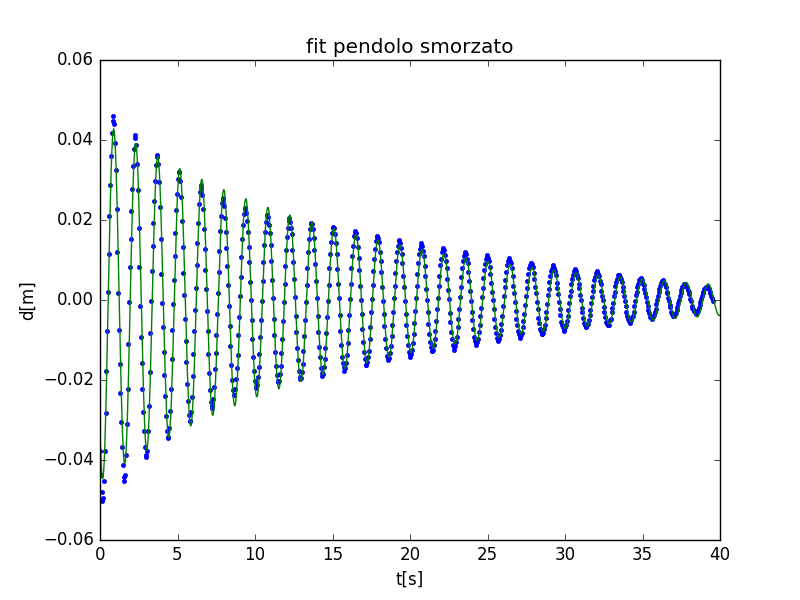
\includegraphics[width=\textwidth]{fit_smorzato}
				\end{minipage}
			\begin{minipage}{0.5\textwidth}
				\begin{tabular}{ll}
					\toprule
					Dati & Parametri ottimali \\
					\midrule
					$\tau_{0}[\textrm{s}]$ & $16,24 \pm 0,02$ \\
					$A_{0}[\textrm{cm}]$ & $4,51 \pm 6,01(10^{-6})$\\
					$\omega_{0}[\textrm{s}^{-1}]$ & $4,42 \pm 2,7(10^{-7})$\\			
					$\phi_{0}$ & $3,94 \pm 3,16$\\
					\bottomrule

				\end{tabular}
			\end{minipage}
			Si osservi che i punti sperimentali non seguono perfettamente una curva esponenziale, poich\'e il modello teorico non tiene in considerazione distubi esterni come l'attrito del perno e rumore esterno, e a causa di ci\'o il chi quadro risulta enorme, tuttavia la precisione sull'ampiezza e sul periodo \'e comunque parecchio elevata

		%In fase ---------------------------------------------------------------------------
			\subsection{Pendoli in fase}
			In seguito abbiamo raccolto i dati degli oscillatori in fase, come si pu\'o notare $\omega_{1}$ che $\tau_{1}$ sono praticamente uguali a $\omega_{0}$ e $\tau_{0}$ , questo perch\'e la molla resta alla sua posizione di riposo e quindi \'e come se non ci fosse\\
			\begin{minipage}{0.5\textwidth}
				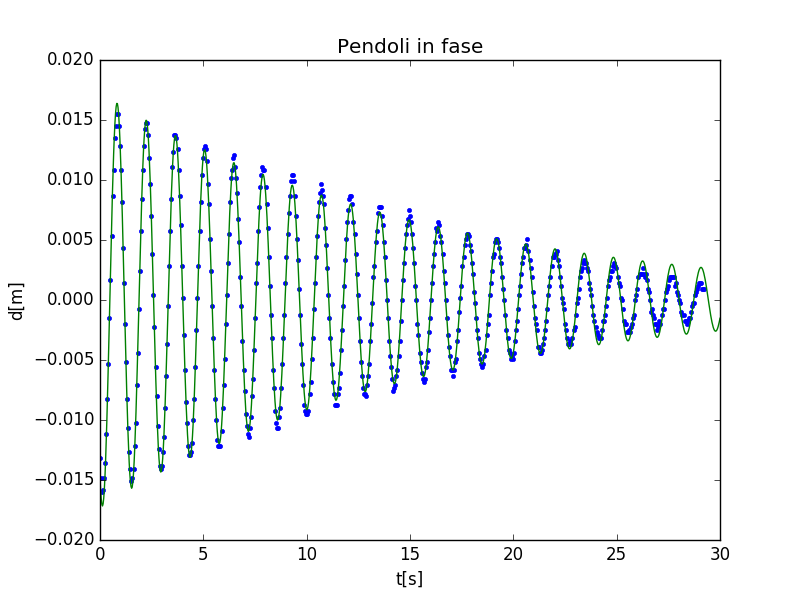
\includegraphics[width=\textwidth]{fase}
			\end{minipage}
			\begin{minipage}{0.5\textwidth}
				\begin{tabular}{ll}
					\toprule
					Dati & Parametri ottimali \\
					\midrule
					$\tau_{f}[\textrm{s}]$ & $15,72 \pm 0,02$ \\
					$A_{f}[\textrm{cm}]$ & $17,29 \pm 6,75(10^{-7})$\\
					$\omega_{f}[{\textrm{s}^{-1}}]$ & $4,17 \pm 2,41(10^{-5})$\\			
					$\phi_{f}$ & $4,45 \pm 2,63(10^{-7})$\\
					\bottomrule
				\end{tabular}
			\end{minipage}
			In questo grafico abbiamo traslato il centro dell'oscillazione a 0, perch\'e la molla spostava la posizione d'equilibrio verso l'altro pendolo, inoltre abbiamo messo solo il grafico di uno dei due pendoli, visto che inserire l'altro risultava ridondante

		%In controfase ---------------------------------------------------------------------
		\subsection{Pendoli in controfase}
			Prima di effettuare la misura dei battimenti abbiamo fatto quella dei pendoli in controfase cosicch\'e ottiniamo i valori di $\omega_{c}$ per verificare che ci\'o che \'e scritto nei cenni teorici\\
			\begin{minipage}{0.5\textwidth}
				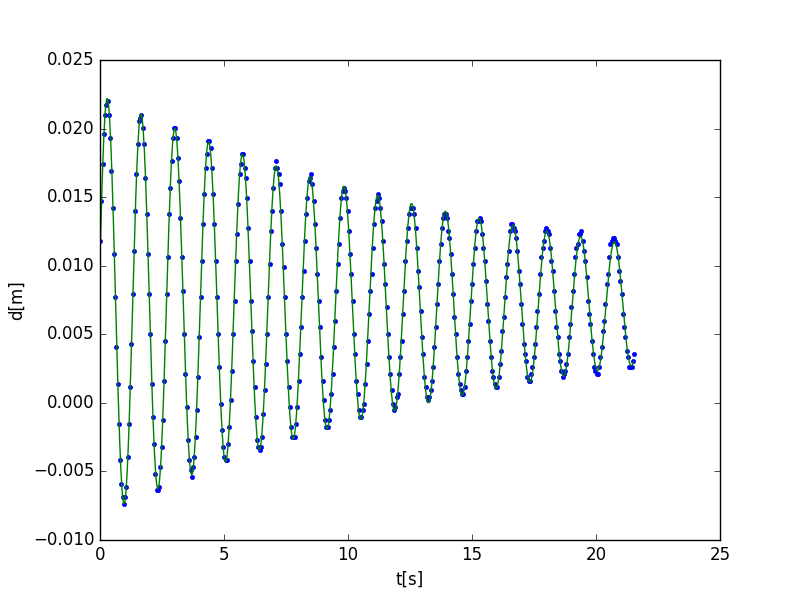
\includegraphics[width=\textwidth]{controfase}
				\end{minipage}
			\begin{minipage}{0.5\textwidth}
				\begin{tabular}{ll}
					\toprule
					Dati & Parametri ottimali \\
					\midrule
					$\tau_{c}[\textrm{s}]$ & $17,27 \pm 0,03$ \\
					$A_{c}[\textrm{cm}]$ & $1,53 \pm 4,89(10^{-7})$\\
					$\omega_{c}[{\textrm{s}^{-1}}]$ & $6,51 \pm 2,11(10^{-5})$\\			
					$\phi_{c}$ & $4,61 \pm 2,87(10^{-7})$\\
					\bottomrule
				\end{tabular}
			\end{minipage}
			La prima cosa che salta all'occhio \'e che $\omega$ \'e aumentato come si ci aspettava, mentr $\tau$ non cambia di molto \'e
		%Battimenti ------------------------------------------------------------------------
		\subsection {Battimenti}
			Dulcis in fundu, abbiamo fatto la raccolta dati dei battimenti e fatto il fit. Questo fit \'e risultato parecchio impegnativo perch\'e sembrava non voler trovare il minimo $\chi^2$, ma alla fine cel'abbiamo fatta.\\
			\begin{minipage}{0.5\textwidth}
				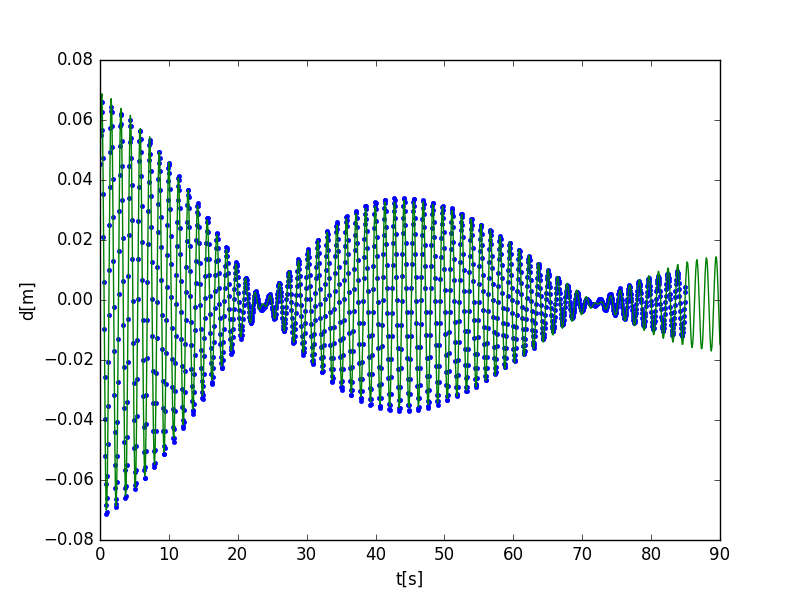
\includegraphics[width=\textwidth]{Battimenti}
				\end{minipage}
			\begin{minipage}{0.5\textwidth}
				\begin{tabular}{ll}
					\toprule
					Dati & Parametri ottimali \\
					\midrule
					$\tau[\textrm{s}]$ & $64,30 \pm 0,09$ \\
					$A[\textrm{cm}]$ & $7,05 \pm 5,67(10^{-7})$\\
					$\omega_{a}[\textrm{s}^{-1}]$ & $4,51 \pm 4,70(10^{-9})$\\
					$\omega_{b}[\textrm{s}^{-1}]$ & $6,48 \pm 6,64(10^{-9})$\\			
					$\phi_{a}$ & $2,05 \pm 4,37(10^{-6})$\\
					$\phi_{b}$ & $3,19 \pm 9,50(10^{-6})$\\
					\bottomrule
				\end{tabular}
			\end{minipage}
			dalla lettura dei dati si ci accorge che $\omega_{a}$ \'e molto simile a $\omega_{f}$ e $\omega_{b}$ a $\omega_{c}$, ci\'o \'e previsto dalla teoria.
	\section{Conclusione}
		La raccolta dati ci conferma che il modello teorico \'e corretto anche se il $\chi^2$ risulta straordinariamente alto (nell'ordine dei milioni) e il p-value viene 0 spaccato


\end{document}